\subsection{Generalities}

Eye tracking is the process of measuring either the point of gaze (where one is looking) or the motion of an eye relative to the head. An eye tracker is a device for measuring eye positions and eye movement. There are a number of methods for measuring eye movement. The most popular variant uses video images from which the eye position is extracted. Other methods use search coils or are based on the electrooculogram.

In the 1950s, Alfred L. Yarbus did important eye tracking research and his 1967 book is often quoted. He showed the task given to a subject has a very large influence on the subject's eye movement. He also wrote about the relation between fixations and interest.

"Records of eye movements show that the observer's attention is usually held only by certain elements of the picture.... Eye movement reflects the human thought processes; so the observer's thought may be followed to some extent from records of eye movement (the thought accompanying the examination of the particular object). It is easy to determine from these records which elements attract the observer's eye (and, consequently, his thought), in what order, and how often."

In 1980, Just and Carpenter formulated the influential \textbf{Strong eye-mind hypothesis}, that "there is no appreciable lag between what is fixated and what is processed". If this hypothesis is correct, then when a subject looks at a word or object, he or she also thinks about it (process cognitively), and for exactly as long as the recorded fixation. 

Comment mesurer la position de l'oeil?

\begin{itemize}
\item Electro-oculogramme: la r\'etine est charg\'ee n\'egative et la corn\'ee positivement. La diff\'erence de potentiel indique la direction. Ceci fonctionne aussi yeux ferm\'es, par exemple pour l'\'etude du sommeil.

\begin{figure}[H]
\centering
\makebox[\textwidth][c]{
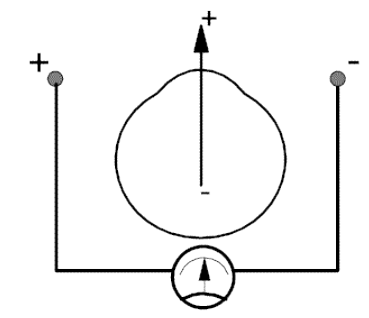
\includegraphics[scale=0.55]{./images/electro.png}
}
\end{figure}

\item M\'ethodes optiques: on projette une lumière infrarouge sur l'oeil. Ceci augmente le contraste pupille-iris. La lumi\`ere se refl\`ete sur la r\'etine et illumine la pupille si l'orientation de l'oeil est coaxiale \`a la cam\'era, moins si l'oeil s'\'eloigne de l'axe. 

Calibration: on associe le centre de la pupille \`a des points distribu\'es  sur l'\'ecran. Des cam\'eras d\'etectent la r\'eflexion sur la corn\'ee (GLINT), lesquelles indiquent la position de la t\^ete vis-\`a-vis de la cam\'era.

La pr\'ecision est une valeur tr\`es controvers\'ee qui d\'epend de la distance de l'utilisateur, de ses mouvements, des conditions d'\'eclairage,....

La pr\'ecision d'un eye tracker est d'environ 1/10 \`eme de la vision fov\'eale. En gros, on est capable de d\'etecter quel caract\`ere est lu.

On peut am\'eliorer la précision par la post-calibration, c'est-\`a-dire mettre a posteriori en correspondance les \'el\'ements regardables et les positions du regard.
\end{itemize}

Les mouvements oculaires sont-ils si rapides?

\begin{itemize}
\item Fixations: 120 - 1000 ms. En général entre 200 et 600. R\'ep\'et\'e 3 fois par seconde.
\item Saccades: sauts rapides de l'oeil entre 40 et 120 ms. Nous sommes aveugles pendant ces moments.
\end{itemize}

\subsection{Applications}

\begin{itemize}
\item Recherche: perception, cognition, education,...Est-ce que montrer la main de l'enseignant permet de guider le regard de l'\'etudiant?
\item Marketing : quels éléments visuels accrochent? Online, TV, panneaux publicit\'e ou rayons dans le supermarch\'e.
\item S\'ecurit\'e: d\'etecter les pertes d'attention par exemple dans la conduite d'un v\'ehicule.
\item Education: d\'etecter le niveau d'expertise par exemple pour le m\'edecins on peut mesurer les mouvements de l'oeil lorsqu'ils r\'egardent une radiographie pendant des secondes. (analytics)
\item Groupware: d\'etecter la qualit\'e de l'interaction.

Collaborative software or groupware is an application software designed to help people involved in a common task to achieve their goals. One of the findings of the Chili lab can be found in this \url{http://chili.epfl.ch/page-92265-en.html} webpage. 

\begin{figure}[H]
\centering
\makebox[\textwidth][c]{
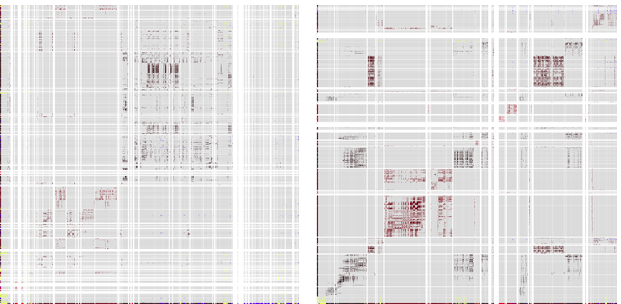
\includegraphics[scale=0.55]{./images/cross.png}
}
\end{figure} 

Cross-recurrence is a general way to explore the coupling between two dynamical systems. In cross-recurrence plots like the ones shown above, each axis is the timeline of one system and the colored points show whether the two systems are in the same state at a given lag in time (the diagonal corresponds to synchronicity). In the context of dual gaze, the dark points on the diagonal represent two people looking at the “same thing” at the “same time”.

\begin{figure}[H]
\centering
\makebox[\textwidth][c]{
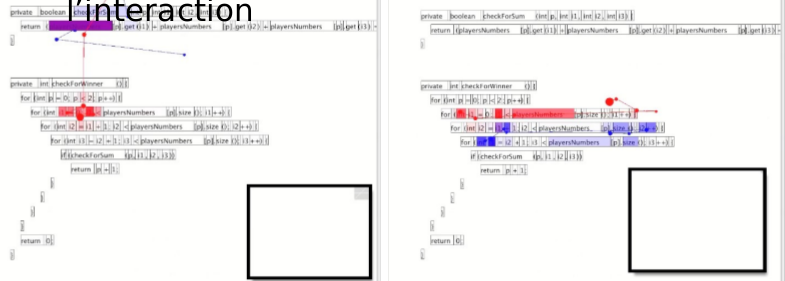
\includegraphics[scale=0.55]{./images/experience.png}
}
\end{figure}

The two cross-recurrence plots above correspond to a 10 minutes long interaction of two programmers reading JAVA code. The graphs are strikingly different. For the dyad on the left, the density of recurrence points on the diagonal is not very marked. The numerous white stripes are indicative of frequent scrolling. For the dyad on the right, clearly defined rectangular areas appear along the diagonal of the plot. This pattern is indicative of gaze coupling, where the two programmers look at the same parts of the code within a few seconds of each other, and hence explore the code together. We have found that high cross-recurrence is one criteria for a good collaboration flow.

\item Contr\^oler une interface avec l'oeil (fonctions): Japanese company NTT DoCoMo has unveiled its new i beam tablet with a a gaze-tracking function that enables users to make selections and turn pages simply by looking at the specific point on the display. 

Prochainement il y aura un eye tracker dans chaque laptop
\item Glasses
\item ...
\item Votre start-up?
\end{itemize}

\subsection{Exercises}

\begin{figure}[H]
\centering
\makebox[\textwidth][c]{
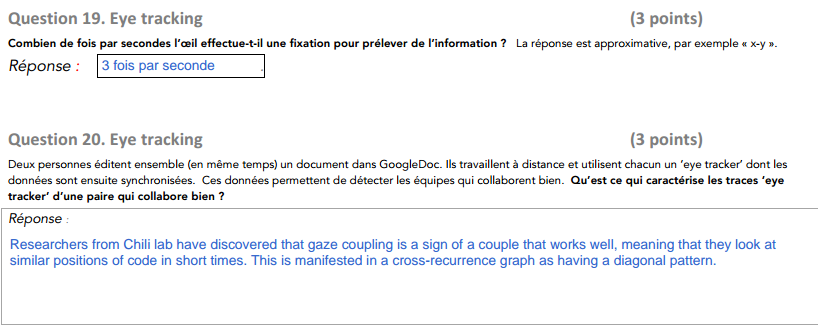
\includegraphics[scale=0.55]{./images/exercise5.png}
}
\end{figure}























